\section{Experiment}
\label{sec:experiment}

Here, we document our \emph{free-market} baseline experiment and illustrate how we collect data such as social welfare, as well as show how skill affects utility. The code below references Python snippets from \texttt{agent.py}, \texttt{utils.py}, etc.

\subsection{Free Market Environment Setup}

We create an environment where no tax component is activated. The config snippet is:

\begin{lstlisting}[language=Python]
env_config = {
    'scenario_name': 'layout_from_file/simple_wood_and_stone',
    'components': [
        ('Build', dict(skill_dist="pareto", payment_max_skill_multiplier=3)),
        ('ContinuousDoubleAuction', dict(max_num_orders=5)),
        ('Gather', dict()),
        # No tax component here
    ],
    'env_layout_file': "quadrant_25x25_20each_30clump.txt",
    'fixed_four_skill_and_loc': True,
    'n_agents': 4,
    'world_size': [25, 25],
    'episode_length': 1000,
    'multi_action_mode_agents': False,
    'multi_action_mode_planner': True,
    'flatten_observations': False,
    'flatten_masks': True,
}
\end{lstlisting}

We then run multiple episodes with random agent actions (for demonstration). We measure social welfare using \texttt{coin\_eq\_times\_productivity}, stored in the environment’s \texttt{previous\_episode\_metrics}.

\subsection{Code for Running the Free Market Simulation}

\begin{lstlisting}[language=Python]
def run_free_market_simulation(num_episodes=50):
    social_welfare_history = []
    for ep in range(num_episodes):
        obs = env.reset()
        done = {'__all__': False}
        
        while not done['__all__']:
            # random actions for now
            actions = sample_random_actions(env, obs)
            obs, rewards, done, info = env.step(actions)
        
        metrics = env.previous_episode_metrics
        swf = metrics.get('social_welfare/coin_eq_times_productivity', np.nan)
        social_welfare_history.append(swf)
        print(f"Episode {ep+1}: SW = {swf}")
    return social_welfare_history
\end{lstlisting}

Using this code, we plot social welfare vs.\ episode index. Figure below shows a typical run of 50 episodes with random policies. The social welfare metric remains relatively unstable due to random play.
\begin{figure}[H]
    \centering
    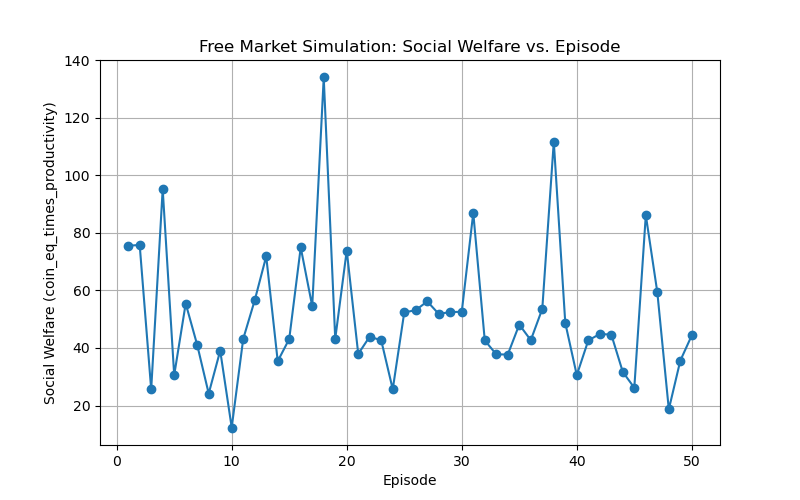
\includegraphics[width=0.6\textwidth]{fig/free_market_sw.png}
    \caption{Free Market Simulation: Social Welfare Over 50 Episodes.}
    \label{fig:free_market_sw}
\end{figure}

\subsection{Utility vs.\ Skill}

Additionally, we analyze how an agent’s skill level (10, 15, 20, 30) interacts with labor performed to yield different utility values, using an isoelastic function. The script \texttt{plot\_and\_save\_utility\_curves} scans labor from $0$ to $1000$ and plots
\[
u(\text{skill}, \text{labor}) = \frac{(\text{income}(\text{skill},\text{labor}))^{1-\eta}-1}{1-\eta} - \text{labor}.
\]
Figure below shows that higher skill yields greater maximum utility at higher labor, with diminishing returns.

\begin{figure}[H]
    \centering
    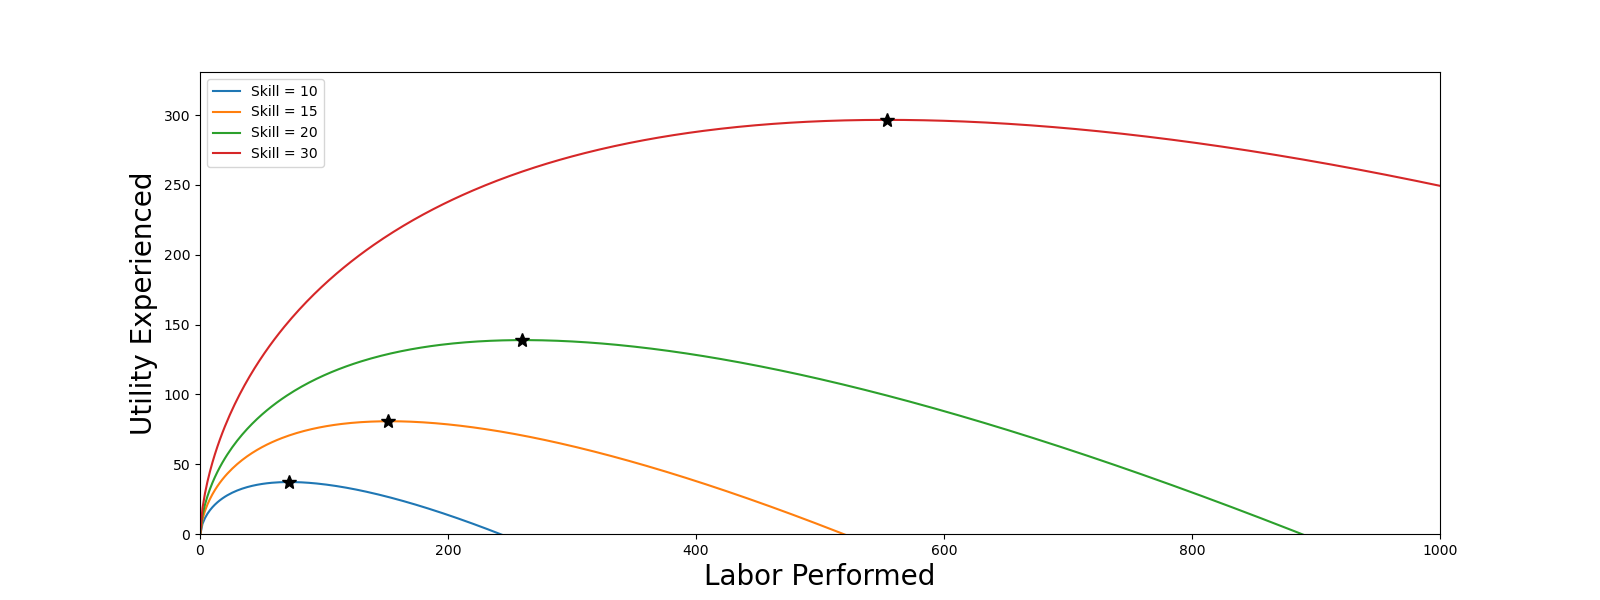
\includegraphics[width=0.6\textwidth]{fig/utility_curves_based_on_skill.png}
    \caption{Isoelastic Utility Curves for Different Skill Levels. Markers indicate the labor level that maximizes the utility at each curve.}
    \label{fig:skill_utility}
\end{figure}

\subsection{Summary of Findings}
\begin{itemize}
    \item Even in a free-market scenario, we see that higher-skill agents can outperform (e.g.\ building) if they invest more labor.
    \item Random actions are not beneficial for social welfare. This underscores the need for a trained policy or carefully guided search.
\end{itemize}
Future experiments will introduce taxes via the \texttt{PeriodicBracketTax} component and compare free-market vs.\ taxed outcomes.

